% !TEX encoding = UTF-8 Unicode
%!TEX root = thesis.tex
% !TEX spellcheck = en-US
%%=========================================
\chapter{Background Information}
\label{chapter:background_information}

\section{Genetic Algorithms}
Genetic algorithms \citep{goldberg1989, back1996} are iterative algorithms that can approximate solutions to optimization problems. In such problems, one usually doesn’t know how to construct a good solution, but it is possible to measure how good a solution is. The methods used in genetic algorithms are inspired by Darwin's principle of natural selection. In the algorithm, a population of individuals is simulated through generations of ``life". Each individual is a candidate solution to the optimization problem. The fittest individuals, as determined by a fitness function, are the individuals that are most likely to survive and reproduce (either asexually or sexually). Individuals that are deemed less fit are more likely to die young, and do not get to pass their genes on to future generations. During reproduction, crossover and mutation occurs. Crossover is a genetic operator that combines two parents to produce an offspring. Mutation is a genetic operator that alters an individual slightly. The whole process is roughly illustrated by figure \ref{fig:genetic_algorithm_cycle}.

\begin{figure}[H]
    \centering
    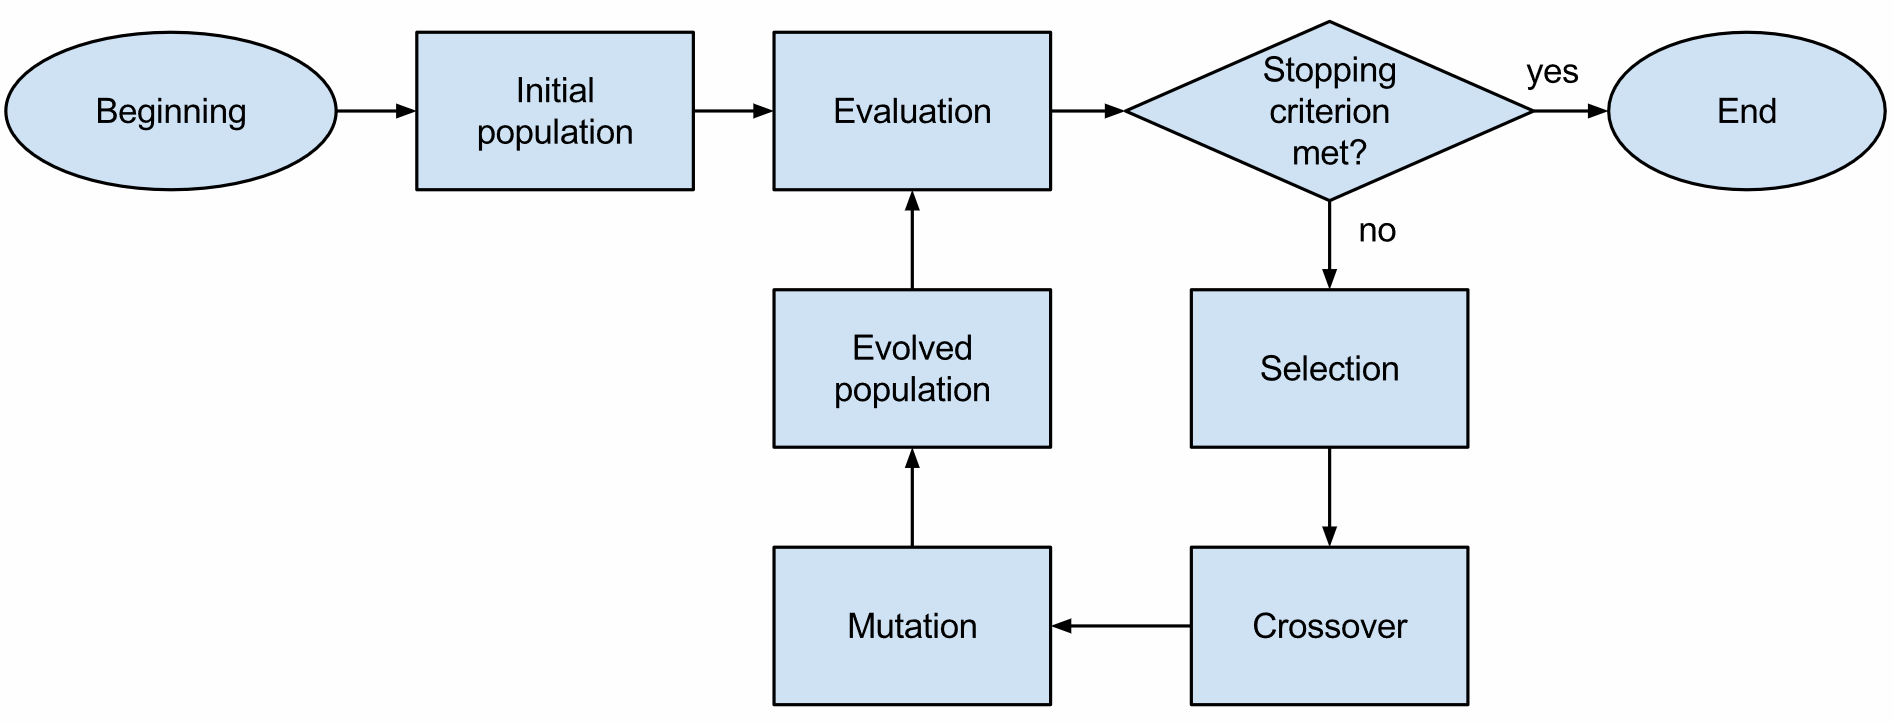
\includegraphics[width=1.0\textwidth]{02_genetic_algorithm_cycle}
    \caption{Genetic algorithm cycle}
    \label{fig:genetic_algorithm_cycle}
\end{figure}

\section{Artificial Neural Networks}
Artificial Neural Networks (ANN) are systems of interconnected ``neurons", or nodes \citep{caudill1987}. A connection from a node A to a different node B means that the activation level of node A influences the activation level of node B based on the numerical weight of the connection. The activation level of a node is calculated by adding up all incoming signals to that node and running that number through the node's activation function. An ANN can be thought of as a function that transforms n-dimensional vectors to m-dimensional vectors. Figure \ref{fig:neural_network} illustrates a simple neural network and the inner workings of one of the nodes.

\begin{figure}[H]
    \centering
    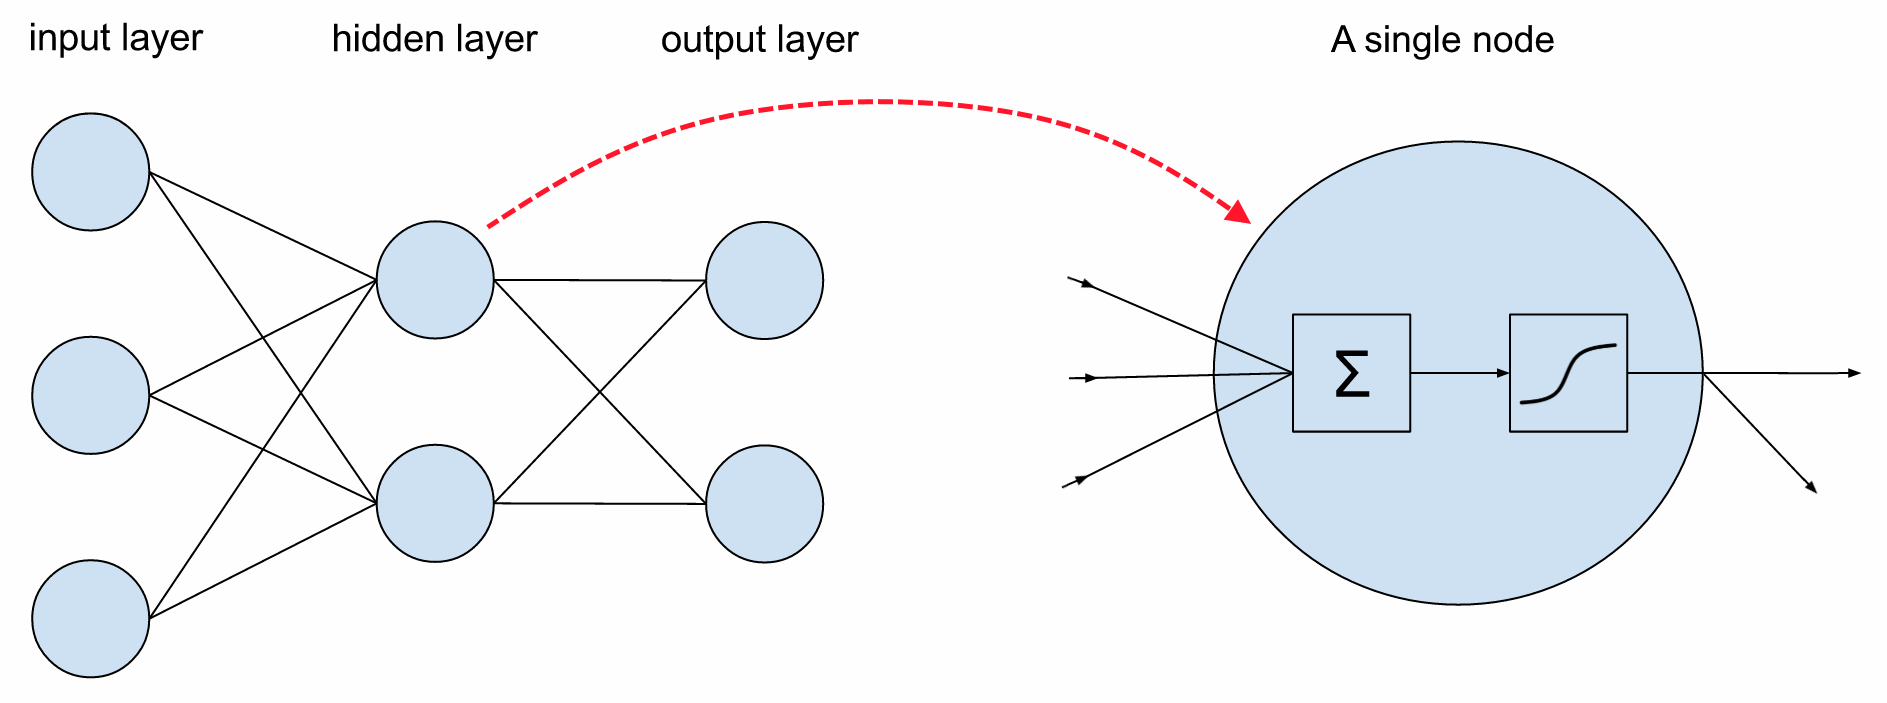
\includegraphics[width=1.0\textwidth]{neural_network}
    \caption{To the left: Illustration of a small neural network with one hidden layer. To the right: Illustration of a hidden node with sigmoid activation function}
    \label{fig:neural_network}
\end{figure}

\section{Neuroevolution}
Neuroevolution is a technique that uses evolutionary algorithms to train artificial neural networks. It differs from supervised learning algorithms such as backpropagation in that it does not require a set of correct input-output pairs. Instead, only a performance measure (fitness function) is needed.

\section{NeuroEvolution of Augmenting Topologies (NEAT)}
NEAT \citep{stanley2002} is a neuroevolution technique that evolves neural networks with genetic algorithms. Not only the weights of the ANN are evolved, but also the structure. The NEAT approach begins with a feed-forward approach with input nodes and output nodes that are fully connected. The ANN can then grow larger by having nodes and links added to it. NEAT can also remove nodes and links.

\iffalse
TODO:
Competing conventions
Species
Genotype (list of nodes, list of connections)
Phenotype
Crossover
Interspecies crossover
Dynamic compatibility
Min species
Max species
Aging species
Innovations
Young age fitness boost
Species stagnation
Competitive coevolution stagnation
Kill worst species each 15 generations
Survival rate
Elitism
Tournament selection
Sexual vs asexual reproduction?
Mutation operations
\fi

\section{Multi-Objective Evolutionary Algorithms}
As real-life problems often have more than one objective, there is a need for ways to deal with multiple objectives effectively. A multi-objective evolutionary algorithm (MOEA) is an algorithm for solving mathematical optimization problems involving more than one objective function to be optimized simultaneously \citep{veldhuizen2000}. One well-known algorithm of this kind is Nondominated Sorting Genetic Algorithm II (NSGA-II) \citep{nsga2}. In this algorithm, the performance measure is based primarily on rank and secondarily on crowding distance. Rank is calculated by running the fast non-dominated sort algorithm. This algorithms assigns a rank to each individual. If the rank of individual A is better than the rank of another individual B, it means that A dominates B. Individual A dominates B if both the following conditions are true:

\begin{itemize}  
\item The solution A is no worse than B in all objectives.
\item The solution A is strictly better than B in at least one objective.
\end{itemize}

Crowding distance is a way to measure how crowded the search space around the individual is. Crowding distance is quantified by forming a cuboid with the nearest neighbours as vertices, and then taking the average of the side lengths of the cuboid. Large crowding distances are encouraged because it preserves diversity in the population \citep{nsga2}.

\section{Audio Feature Extraction Tools}
Audio feature extraction is the process of computing a compact numerical representation that can be used to characterize a segment of audio. Low-level features such as spectral centroid and Mel-Frequency Cepstral Coefficients (MFCC) \citep{mermelstein1976, logan2000} are computed directly from the audio signal, frame by frame. A frame is a slice of audio and can consist of for example 1024 samples. In an audio signal with sampling rate 44.1 kHz, the duration of such a frame would be approximately 23 ms.

Audio features can be used in many different ways, such as music information retrieval and musical genre classification. In this project, they are used for similarity measures and for controlling the parameters of audio effects. Four audio feature extraction tools were used in this project: Aubio \citep{brossier2003aubio}, Essentia \citep{bogdanov2013essentia}, LibXtract \citep{bullock2007libxtract} and Csound \citep{csound}.

\section{Audio Effects}
Audio effects are processing techniques that alter audio so it sounds different. The following subsections describe the audio effects used in this project.

\subsection{Modified Hyperbolic Tangent}
Modified hyperbolic tangent is a waveshaping function that can model the characteristics of analog distortion, and especially tube distortion \citep{mtanh}. Modified hyperbolic tangent differs from hyperbolic tangent in that one can model the positive and the negative slopes differently. This distortion effect makes the sound ``fuzzier" by adding harmonic components. Figure \ref{fig:modified_hyperbolic_tangent_waveform_and_spectrum} illustrates an example of this.

$$\text{mtanh}(x)=\frac{e^{ax}-e^{-bx}}{e^{cx}+e^{-dx}}$$

\begin{figure}[H]
    \centering
    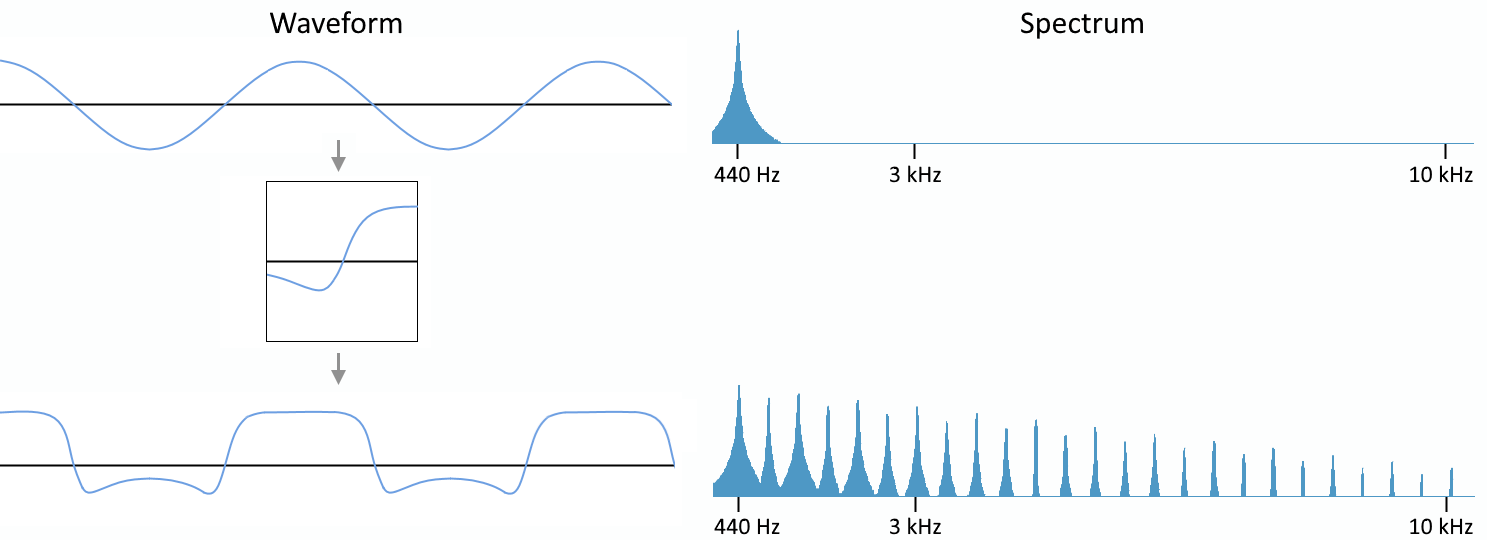
\includegraphics[width=1.0\textwidth]{modified_hyperbolic_tangent_waveform_and_spectrum}
    \caption{Harmonic frequency components are added to a 440 Hz sine wave by applying a modified hyperbolic tangent function}
    \label{fig:modified_hyperbolic_tangent_waveform_and_spectrum}
\end{figure}

\subsection{Low-Pass Filter}
A low-pass filter attenuates high frequencies and retains low frequencies unchanged \citep{dodge_jerse_1997}. It can be used to make a sound ``darker" or ``smoother" in timbre. A resonant low-pass filter is a low-pass filter that has a peak in the response curve at the cutoff frequency, as illustrated by figure \ref{fig:low_pass_filter}. This quality can be used to boost a single tone in a sound with a rich frequency spectrum. The width of the resonant peak is described by a parameter called Q. As Q increases, the resonance becomes more pronounced.

\begin{figure}[H]
    \centering
    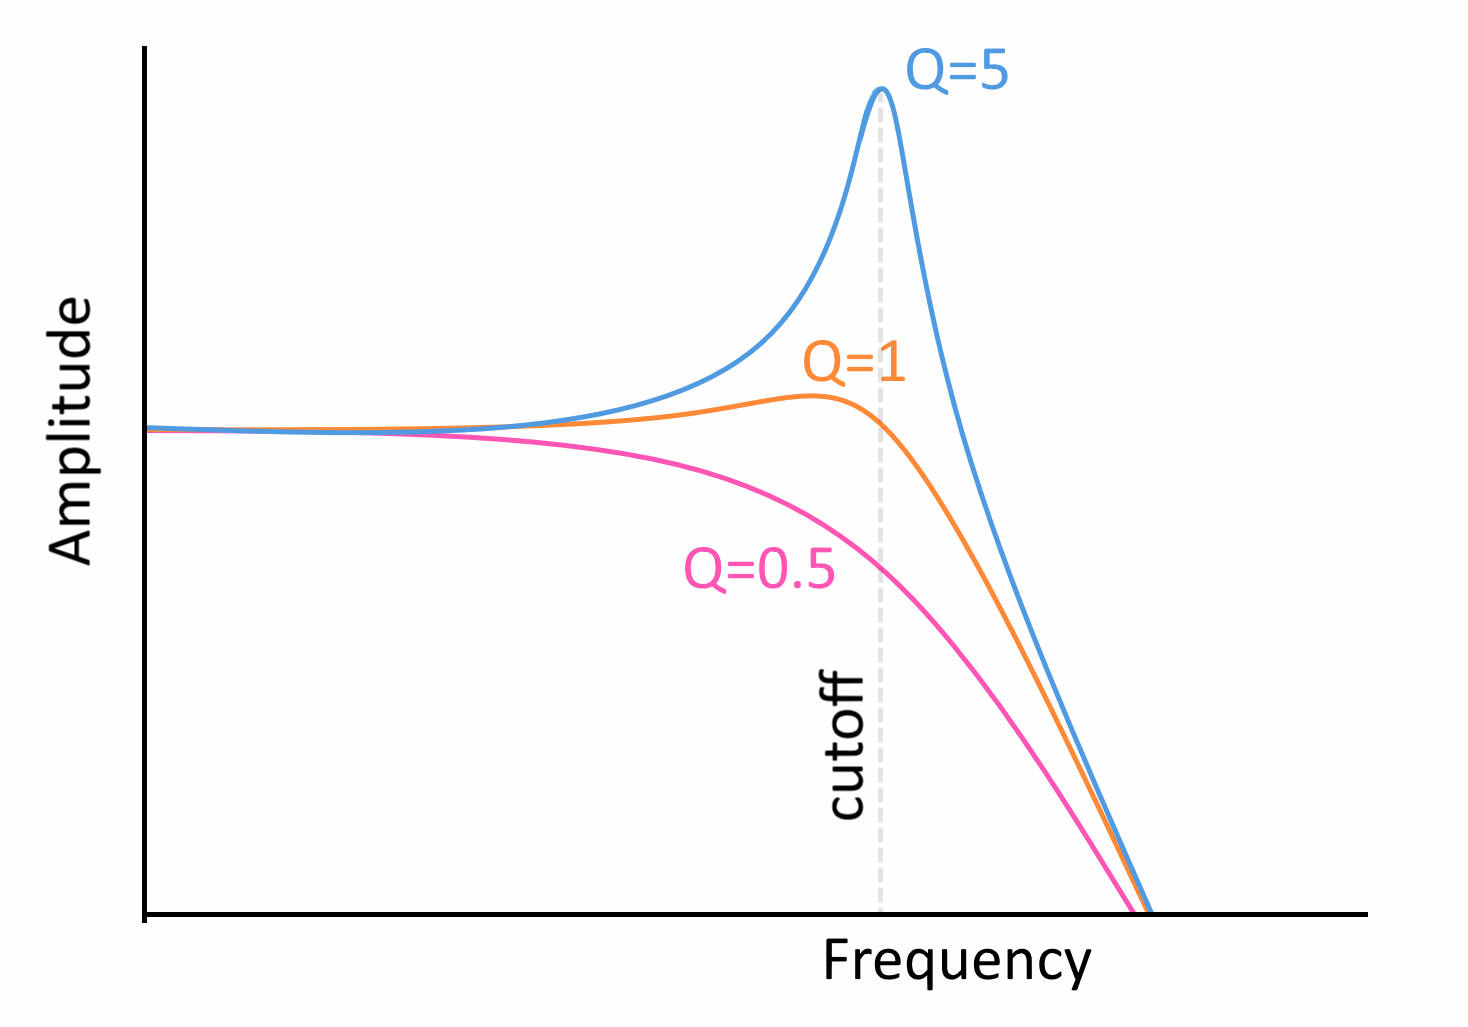
\includegraphics[width=0.5\textwidth]{05_low_pass_filter}
    \caption{Frequency response of a resonant low-pass filter with various Q values}
    \label{fig:low_pass_filter}
\end{figure}

\subsection{Band-Pass Filter}
A band-pass filter rejects frequencies outside a given range \citep{dodge_jerse_1997}. This filter has two parameters. Center frequency (denoted by $f_0$ in figure \ref{fig:bandpass}) defines the center of the frequency range. Bandwidth (denoted by $B$ in figure \ref{fig:bandpass}) defines how broad or narrow the frequency range is.

\begin{figure}[H]
    \centering
    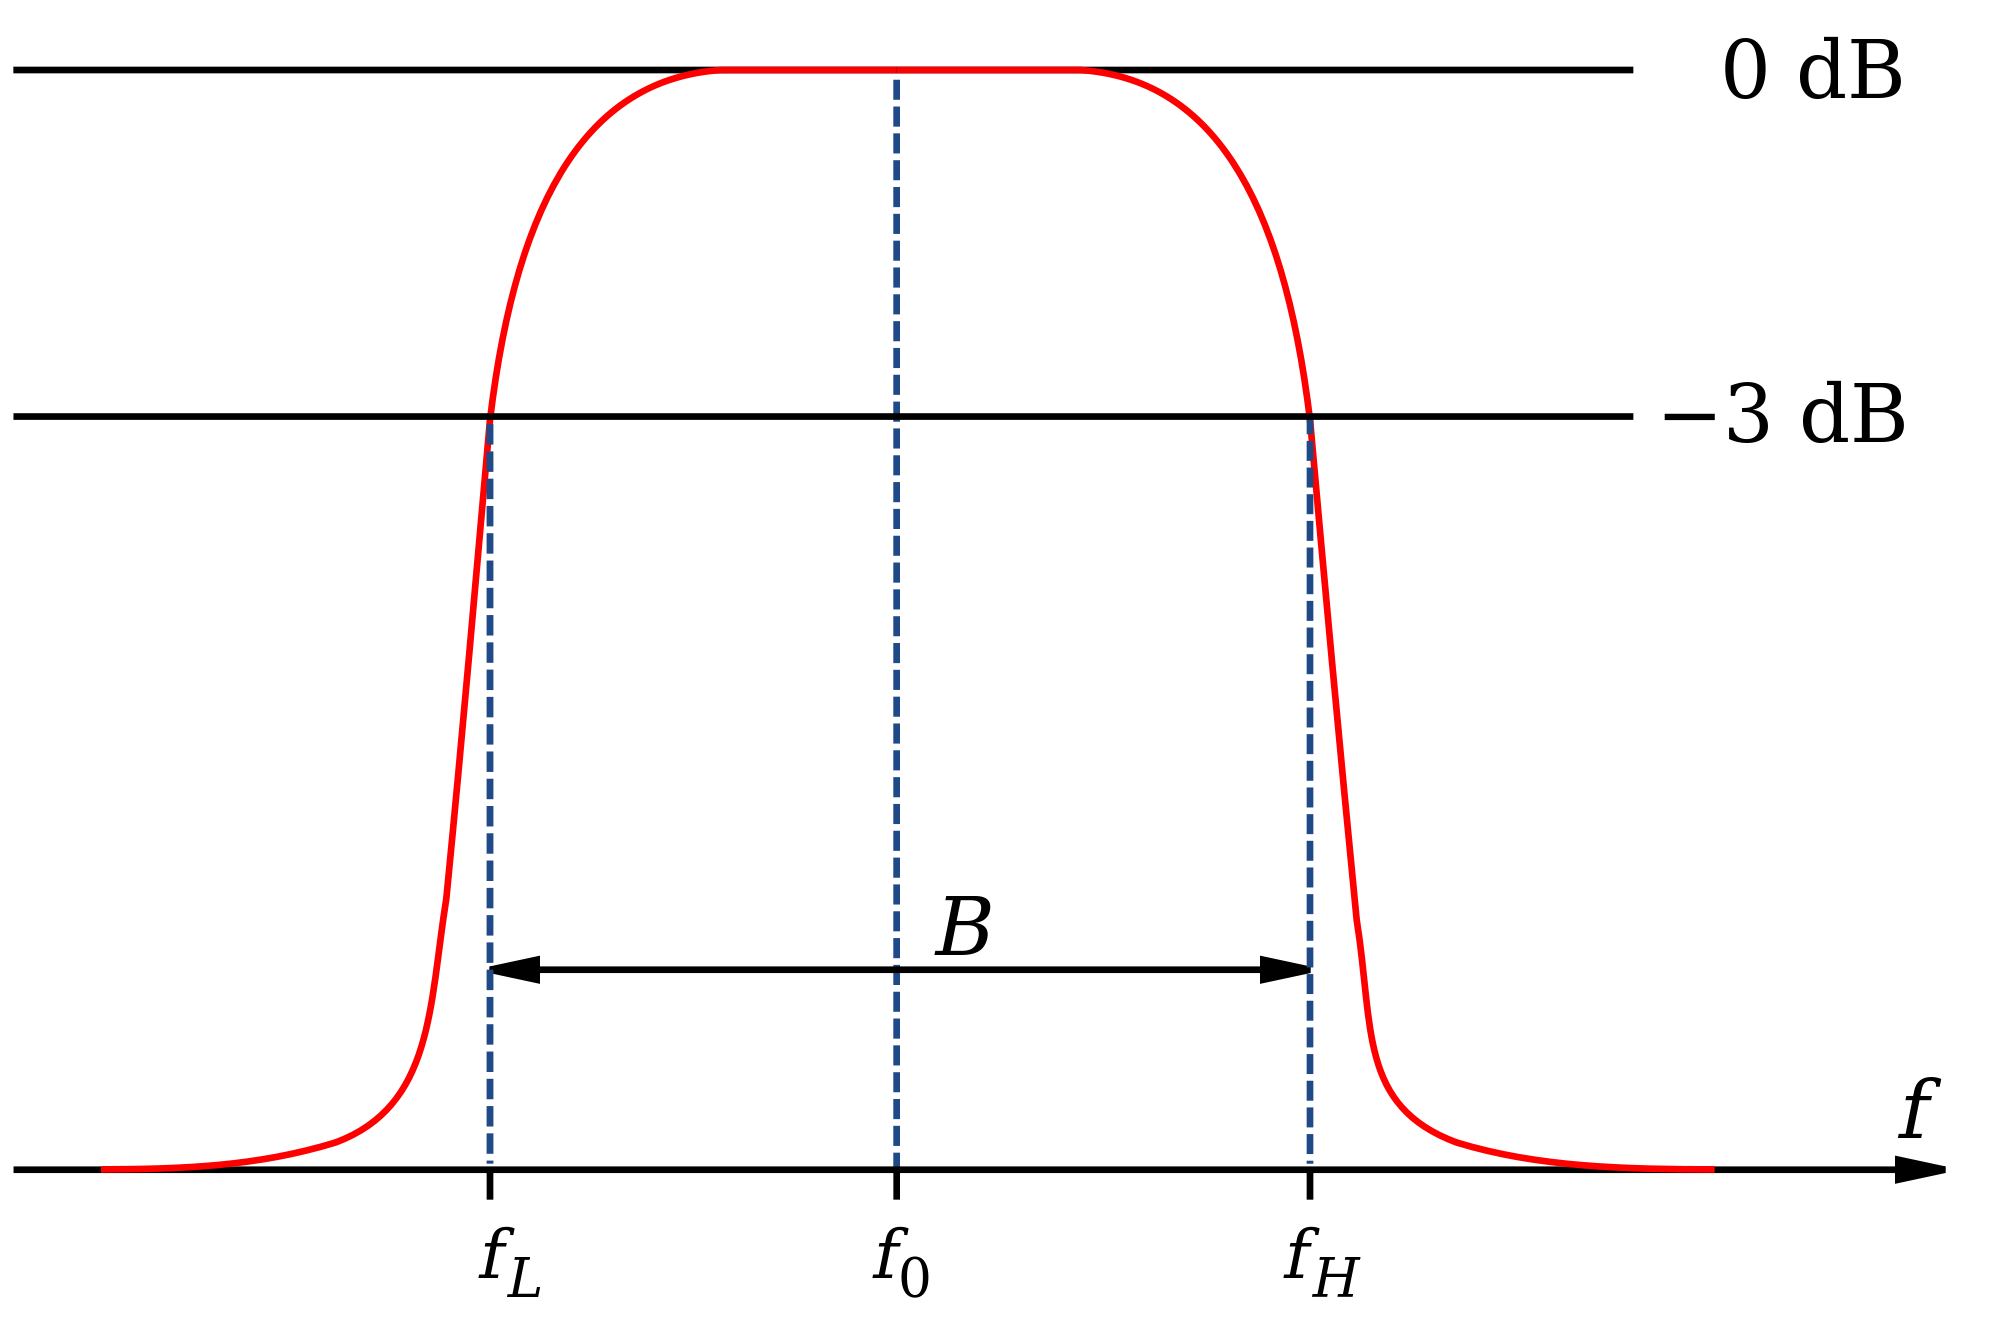
\includegraphics[width=0.5\textwidth]{bandpass}
    \caption{A diagram that illustrates the frequency response of a band-pass filter and defines its bandwidth}
    \label{fig:bandpass}
\end{figure}

\subsection{Amplitude Modulation}
The amplitude modulation effect multiplies the sound signal with a unipolar sine wave that oscillates between 0 and 1. When the frequency of the sine wave is low (\textless~20 Hz), one can hear that the amplitude is being brought up and down, as in tremolo \citep{serafin2007}. With higher frequencies there is instead an effect on the timbre of the sound. The modulator generates a set of frequency sidebands, as illustrated in figure \ref{fig:am_sidebands}

\begin{figure}[H]
    \centering
    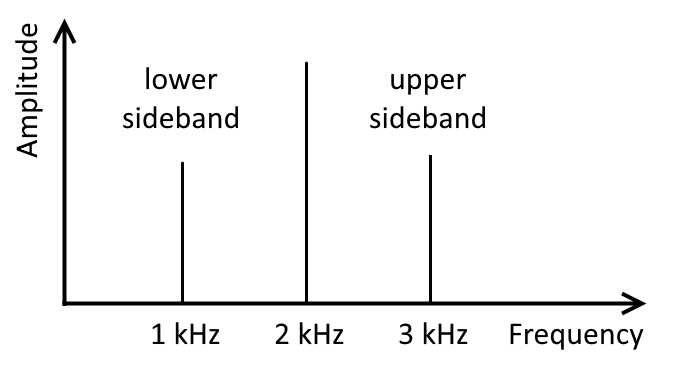
\includegraphics[width=0.5\textwidth]{am_sidebands}
    \caption{Frequency spectrum plot of a 2 kHz sine wave modulated with a 1 kHz unipolar sine wave}
    \label{fig:am_sidebands}
\end{figure}

\subsection{Bit Reduction}
The bit reduction effect reduces the number of bits used to represent a sample \citep{bitreduction}. Each sample amplitude value is rounded to a number of discrete steps. This introduces a particular kind of distortion, also called quantization noise.

\begin{figure}[H]
    \centering
    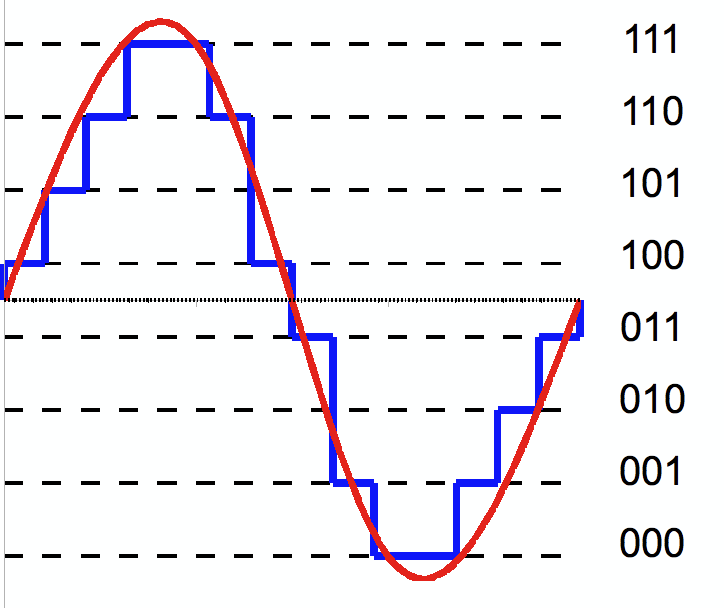
\includegraphics[width=0.3\textwidth]{bit_reduction}
    \caption{A high fidelity sine wave quantized to 3 bits per sample. \textit{By Hyacinth, CC BY-SA 3.0, \url{https://commons.wikimedia.org/w/index.php?curid=30716342}}}
    \label{fig:bit_reduction}
\end{figure}

\subsection{Chorus}
The chorus effect delays the input signal by a short \textit{delay time} (usually in the range 20-50~ms) and mixes it with the dry input signal \citep{chorus}. The \textit{delay time} is variable and usually controlled by a Low-Frequency Oscillator (LFO), as illustrated by figure \ref{fig:chorus}. This may create an impression of multiple voices playing or singing the same thing.

\begin{figure}[H]
    \centering
    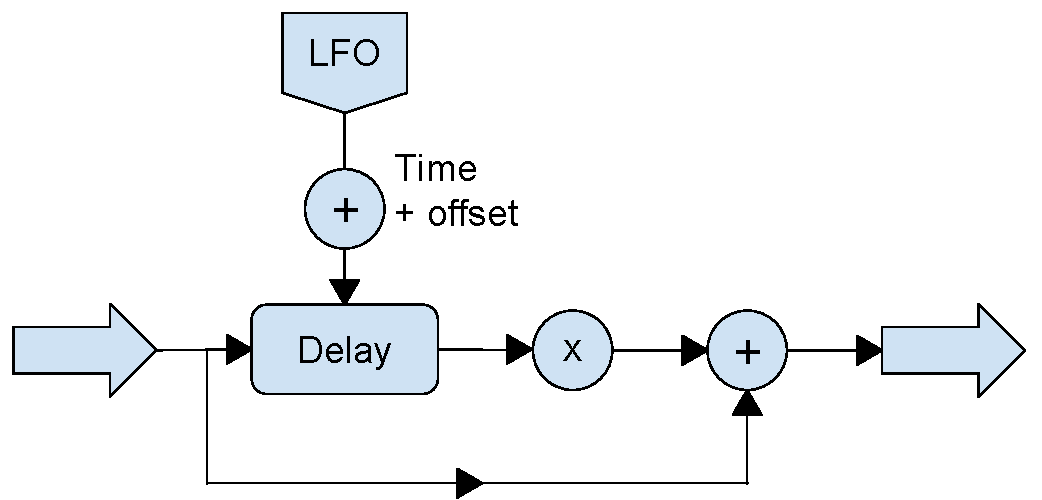
\includegraphics[width=0.5\textwidth]{chorus}
    \caption{Signal flow in a chorus effect}
    \label{fig:chorus}
\end{figure}


\section{Audio Processing Tools}
Audio processing is the alteration of audio signals, typically through audio effects. One popular audio processing tool is Csound \citep{csound}. This is both an audio programming language and a program that runs Csound code. The Csound program takes in a text file of code. This code is executed by the Csound program. The output is sound that is directed to either an audio interface (live) or to a file (non-real-time processing). Csound is used by musicians and composers, typically in experimental electroacoustic music. Traditionally, it has been an offline tool, due to lack of computational power. Today, computational power is sufficient for Csound to run in real-time, so it can be used in live settings such as concerts and sound installations. Csound can not only run on desktop computers, but can also be used as audio processing engine in mobile applications for the operating systems Android and iOS.

\section{Specialization Project}
This master's thesis is a continuation of the author's specialization project. The preliminary experiments in the specialization project were found to be successful. This led to a published paper in the proceedings of the 2nd AES Workshop on Intelligent Music Production\footnote{\url{http://www.aes-uk.org/forthcoming-meetings/wimp2/\#proceedings}}. This paper is included in appendix \ref{appendix:jordal_paper}. The author also presented his findings in a 15-minute talk at this event.

The following subsections will summarize some of the main areas of study in the experiments in the specialization project.

\subsection{Output Activation Functions}
Three different output activation functions (used in the output nodes of the neural networks) were compared. Sigmoid was found to be better than linear and sine in most cases (see figure \ref{fig:output_activation_functions_avg}).

\begin{figure}[H]
    \centering
    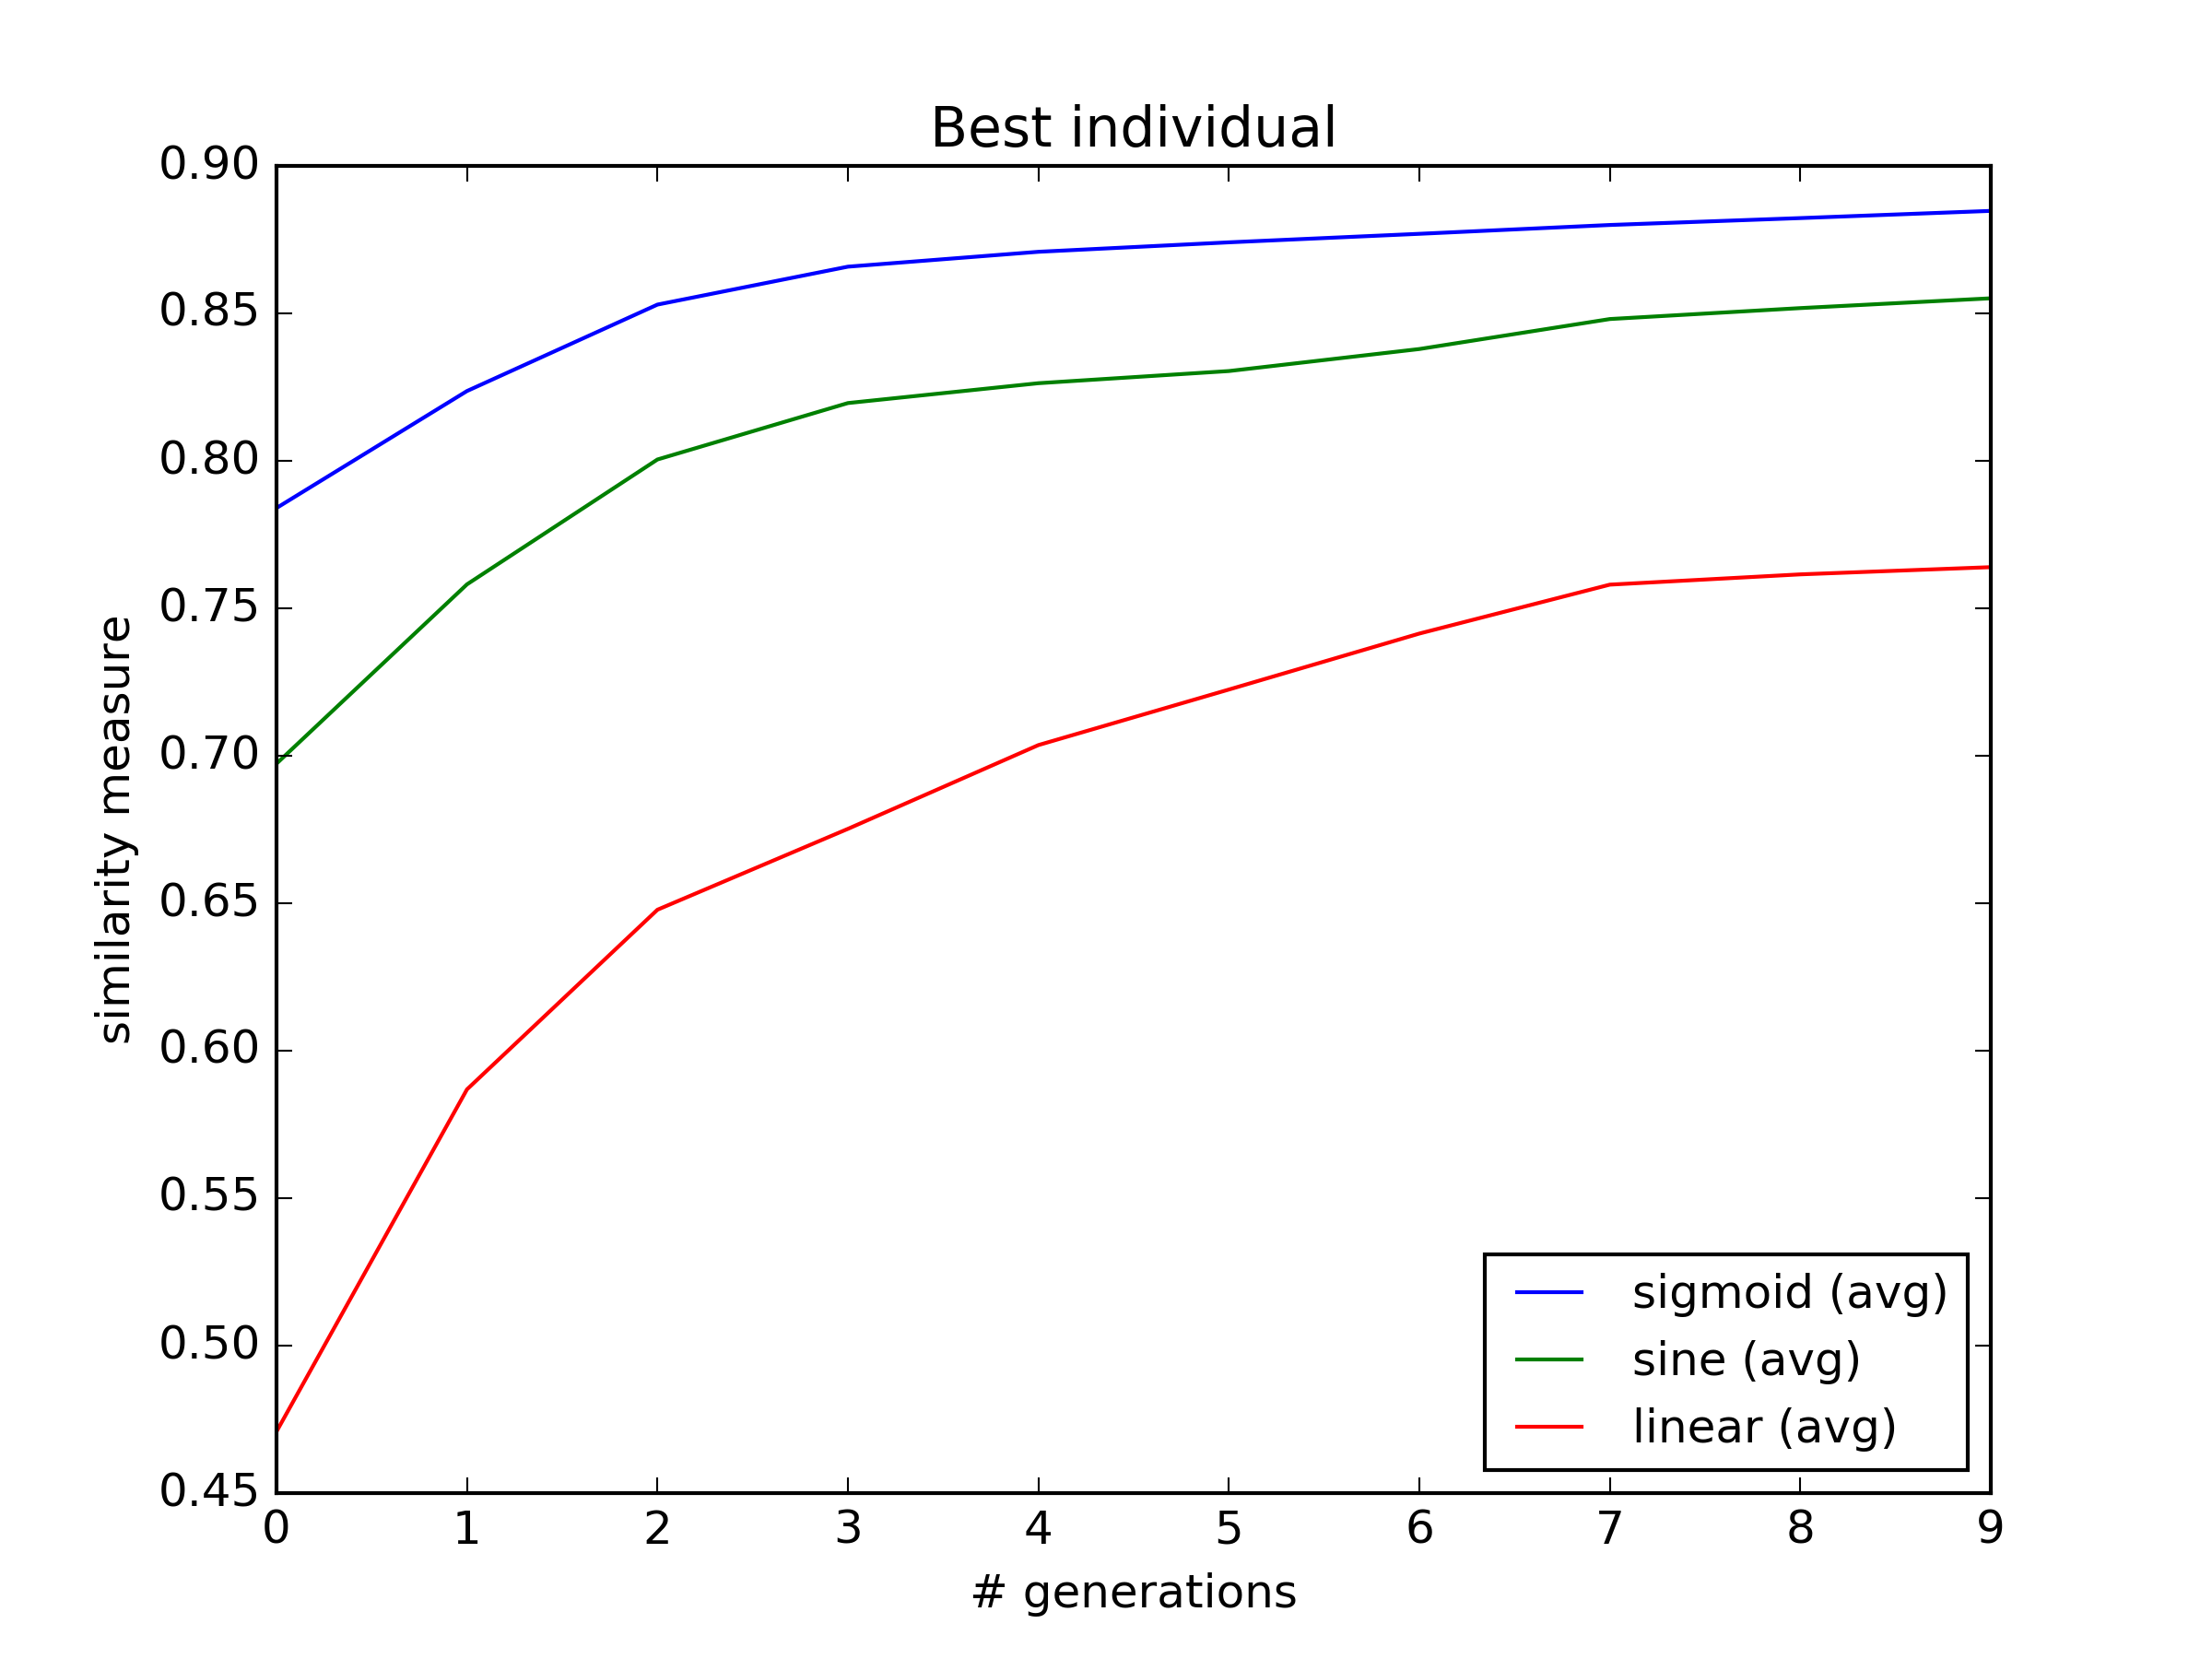
\includegraphics[width=0.85\textwidth]{output_activation_functions_avg}
    \caption{Average fitness over 20 runs. Three different output activation functions are compared.}
    \label{fig:output_activation_functions_avg}
\end{figure}

\subsection{Fitness Functions}
Five fitness functions were compared. Figure \ref{fig:fitness_functions_avg} shows how well they scored on average on the similarity measure (local similarity).

\subsubsection{Local Similarity}
The local similarity fitness function is based on the average euclidean distance between the feature vector of the target sound and the output sound in the k frames of the two sounds.

\begin{verbatim}
Function LOCAL_SIMILARITY(target, individual):
    total_euclidean_distance = 0
    for each k in range(num_frames):
        A = target.get_feature_vector(k)
        C = individual.get_feature_vector(k)
        total_euclidean_distance += EUCLIDEAN_DISTANCE(A, C)
    avg_euclidean_distance = total_euclidean_distance / num_frames
    return 1 / (1 + avg_euclidean distance)
\end{verbatim}

where \texttt{EUCLIDEAN\_DISTANCE} is $d(p,q)=\sqrt{(q_1-p_1)^2+(q_2-p_2)+...+(q_n-p_n)^2}$

\subsubsection{Multi-Objective Optimization}
This fitness function is inspired by NSGA-II \citep{nsga2}. It incorporates two measures: rank and crowding distance. These are concepts taken directly from the NSGA-II paper, and they are then used in a math expression that satisfies these two constraints that are used in NSGA-II:

\begin{itemize}
\item $\text{rank}(A) > \text{rank}(B) \implies \text{fitness}(A) > \text{fitness}(B)$
\item $\text{rank}(A) = \text{rank}(B), \text{CD}(A) > \text{CD}(B) \implies \text{fitness}(A) > \text{fitness}(B)$
\\ where CD stands for crowding distance
\end{itemize}

The ranks of the individual are calculated by doing non-dominated sort. Crowding distance is computed between individuals in a given rank. The multi objective fitness function works like this:

\begin{Verbatim}[fontsize=\small]
Function MULTI_OBJECTIVE(target, individuals):
    for individual in individuals:
        CALCULATE_OBJECTIVES(individual, target)
    fronts = FAST_NON_DOMINATED_SORT(individuals)
    for rank in fronts:
        CALCULATE_CROWDING_DISTANCE(fronts[rank])  # assigns individual.crowding_distance
        for individual in fronts[rank]:
            individual.fitness = 1.0 / (rank + (0.5 / (1.0 + individual.crowding_distance)))

Function CALCULATE_OBJECTIVES(individual, target):
    individual.objectives = {}
    for feature in similarity_features:
        individual.objectives[feature] = EUCLIDEAN_DISTANCE(
                                             target.analysis[feature],
                                             output.analysis[feature])
\end{Verbatim}

Pseudocode for \texttt{FAST\_NON\_DOMINATED\_SORT} and \texttt{CALCULATE\_CROWDING\_DISTANCE} can be found in the NSGA-II paper \citep{nsga2}.

\subsubsection{Hybrid}
While NSGA-II is good at optimizing for non-dominated individuals, these individuals may be extreme tradeoffs and therefore not necessarily feasible solutions in practice. In order to reward good tradeoffs more, the author developed the hybrid fitness function. This fitness function returns the average of \texttt{MULTI\_OBJECTIVE} and \texttt{LOCAL\_SIMILARITY}.

\subsubsection{Novelty Search}
Novelty search \citep{lehman2008} ignores the objective and optimizes for novelty instead. The reason that this may work well is that in some problems the intermediate steps to the goal do not resemble the goal itself. When it comes to implementation, MultiNEAT has novelty search built-in, but Python bindings for it are missing, so the author could not use it in his Python application. However, novelty search can be implemented on top of most evolutionary algorithms, by using a fitness function that rewards novelty \citep{noveltysearchwebsite}, so that is what the author did. First, each individual needs to be represented as a vector that describes its characteristics. This vector is constructed by concatenating all audio feature series of the individual. The implemented fitness function assigns high fitness values to the individuals that have long euclidean distances from the 3 nearest neighbours, where the neighbours are individuals that have been evaluated earlier. The very first population gets random fitness values, because there are no earlier individuals to measure distance from.

\subsubsection{Mixed}
This fitness function is simple: For each generation, one of the following fitness functions is chosen randomly and applied: local similarity, multi-objective, hybrid, novelty. The idea behind this fitness function is to create a dynamic fitness landscape, where the individuals that get good scores from all fitness functions have the greatest chance of survival over time.

\begin{figure}[H]
    \centering
    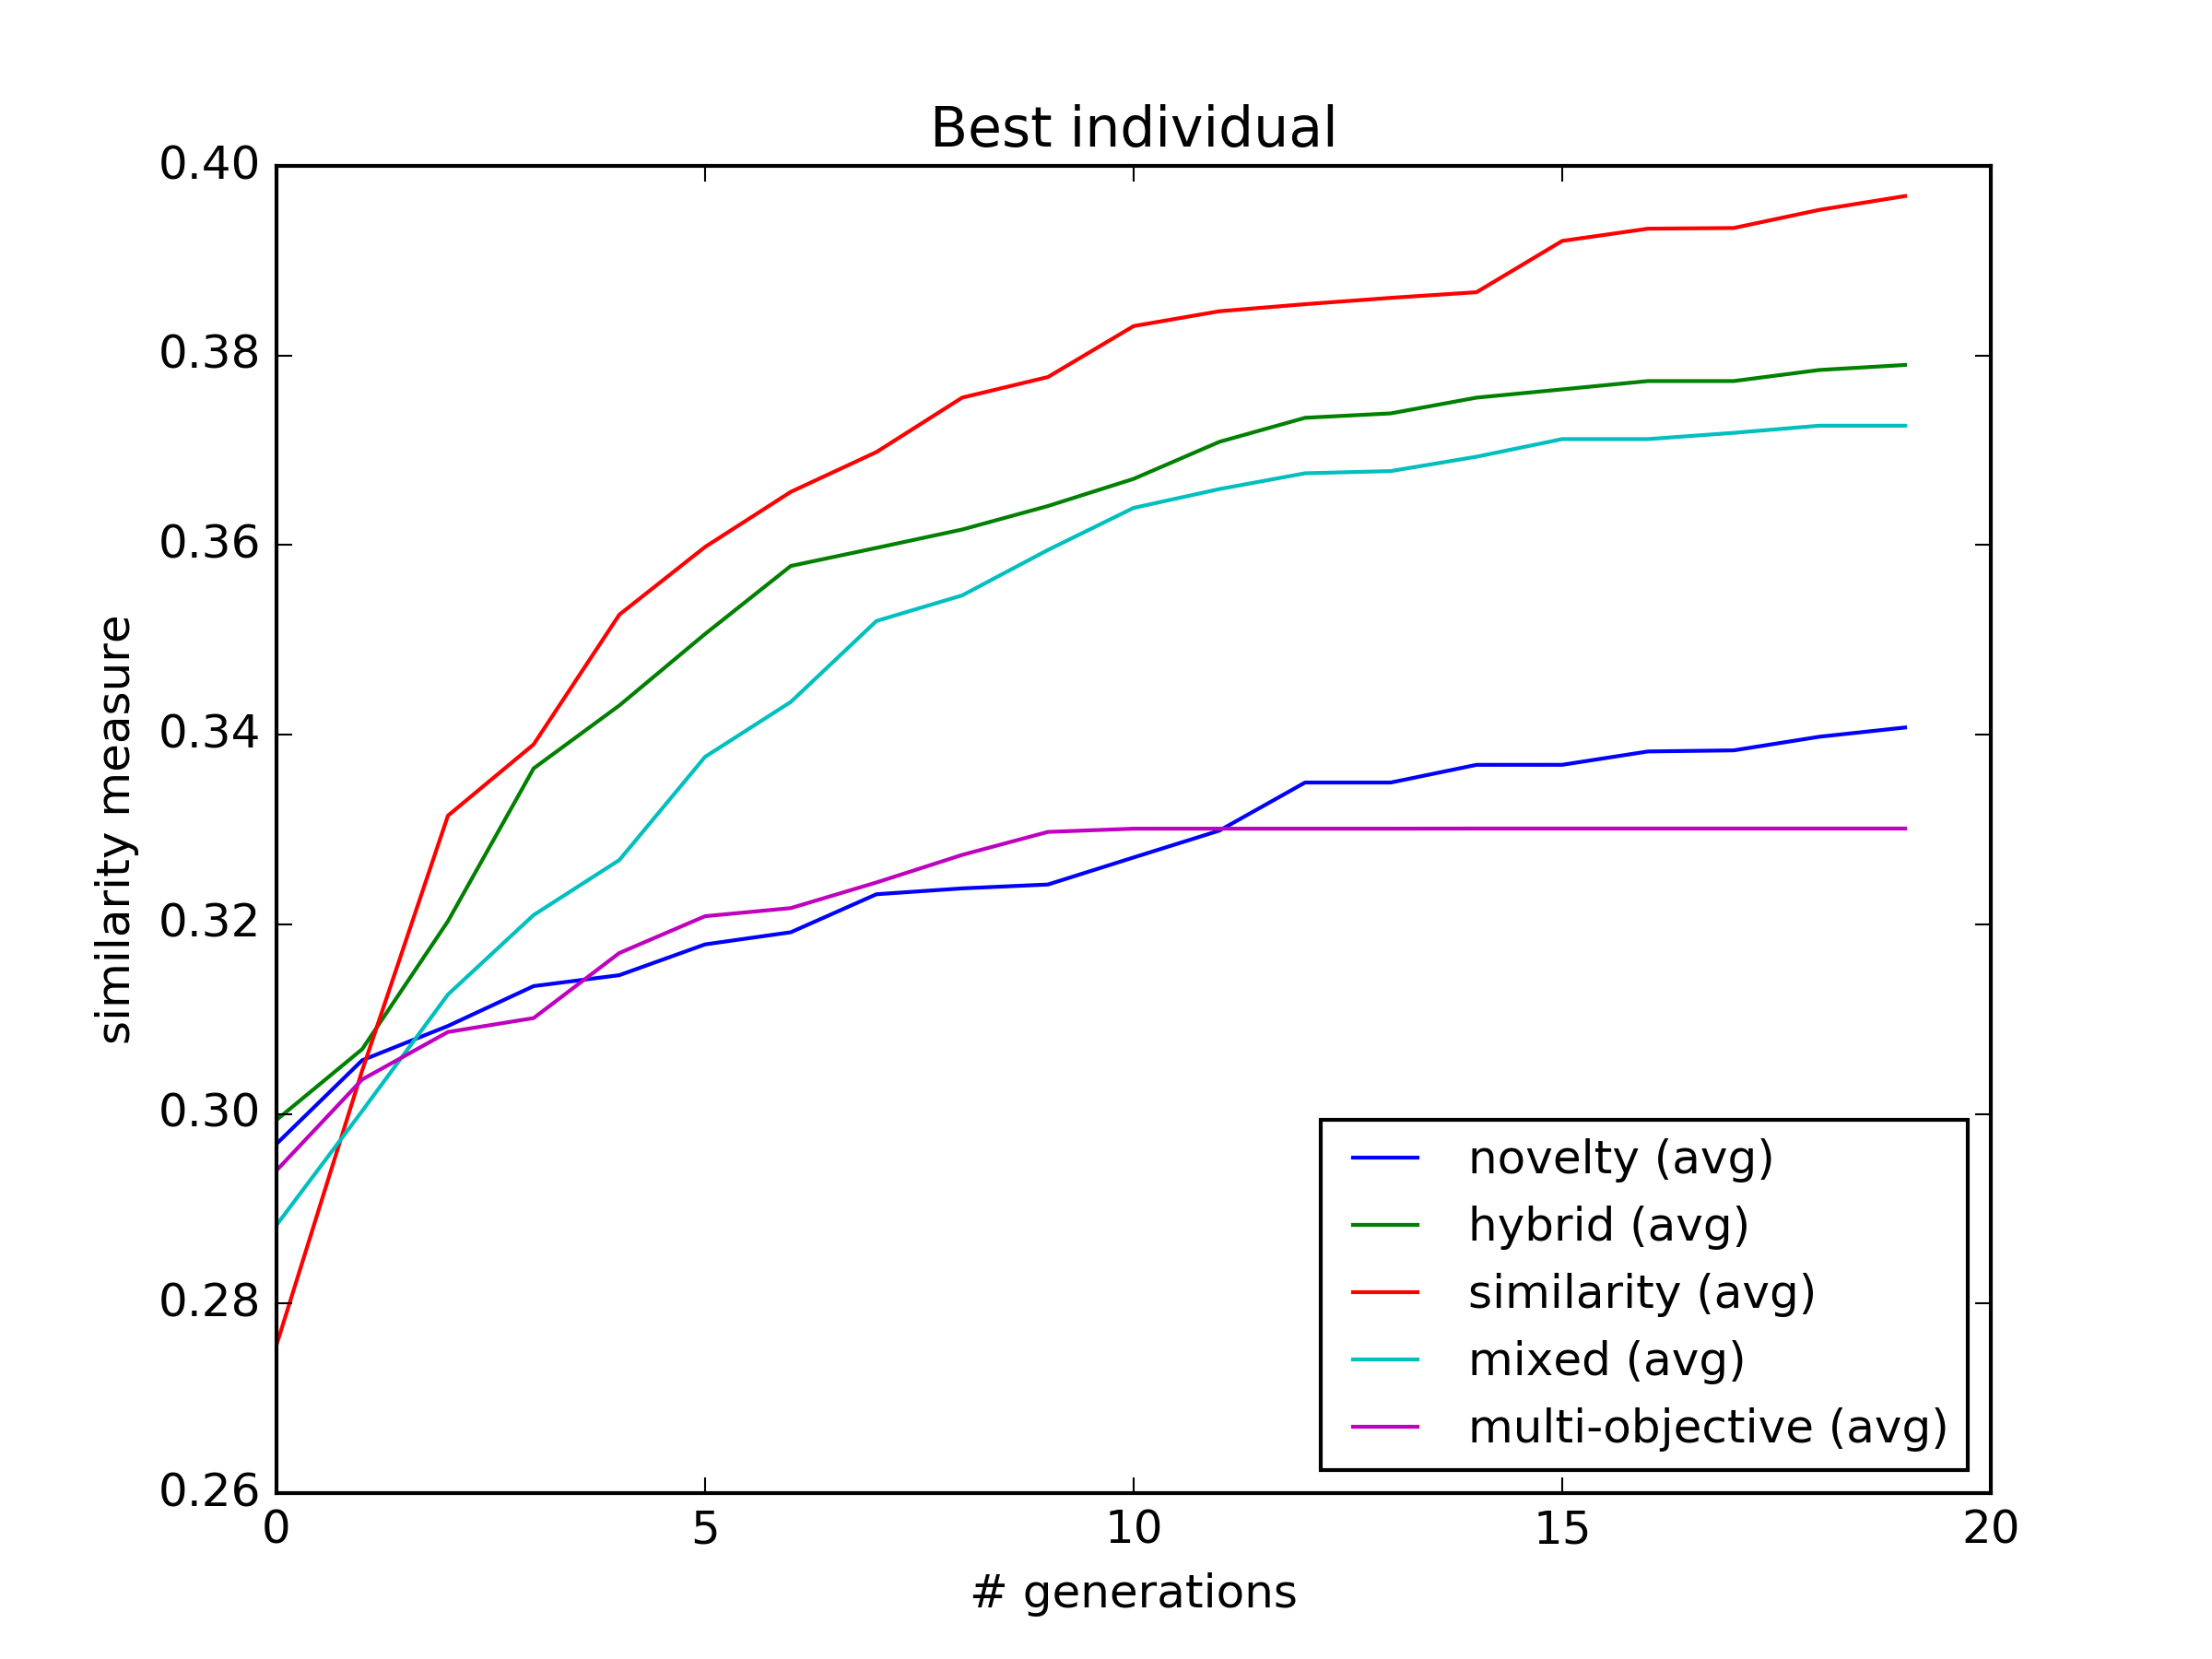
\includegraphics[width=0.85\textwidth]{fitness_functions_avg}
    \caption{Best individual on average over 20 runs, with 20 generations for each run}
    \label{fig:fitness_functions_avg}
\end{figure}

\subsection{Automatic Feature Selection}
When dealing with high-dimensional input data, the number of weights in a fully connected neural network becomes quite large. Clean and useful combinations of all the input signals can be hard to evolve. To deal with this situation, one can use Feature Selective NeuroEvolution of Augmenting Topologies (FS-NEAT) \citep{whiteson2005}. This NEAT variation starts with just a few connections and gradually adds/removes connections.

In an experiment with noise for input sound and a sine sweep for output sound, FS-NEAT was found to perform better than classic NEAT. This experiment had 68 audio features as input. Classic NEAT would typically evolve a very noisy parameter control, so the output sounds became glitchy and not very musically interesting. FS-NEAT has been found to deal with the high-dimensional input more effectively, as it selected only a few of the audio features that were useful for getting high fitness values. Figure \ref{fig:neat_vs_fs_neat_avg_max} shows fitness values with NEAT and FS-NEAT in the described experiment.

\begin{figure}[H]
    \centering
    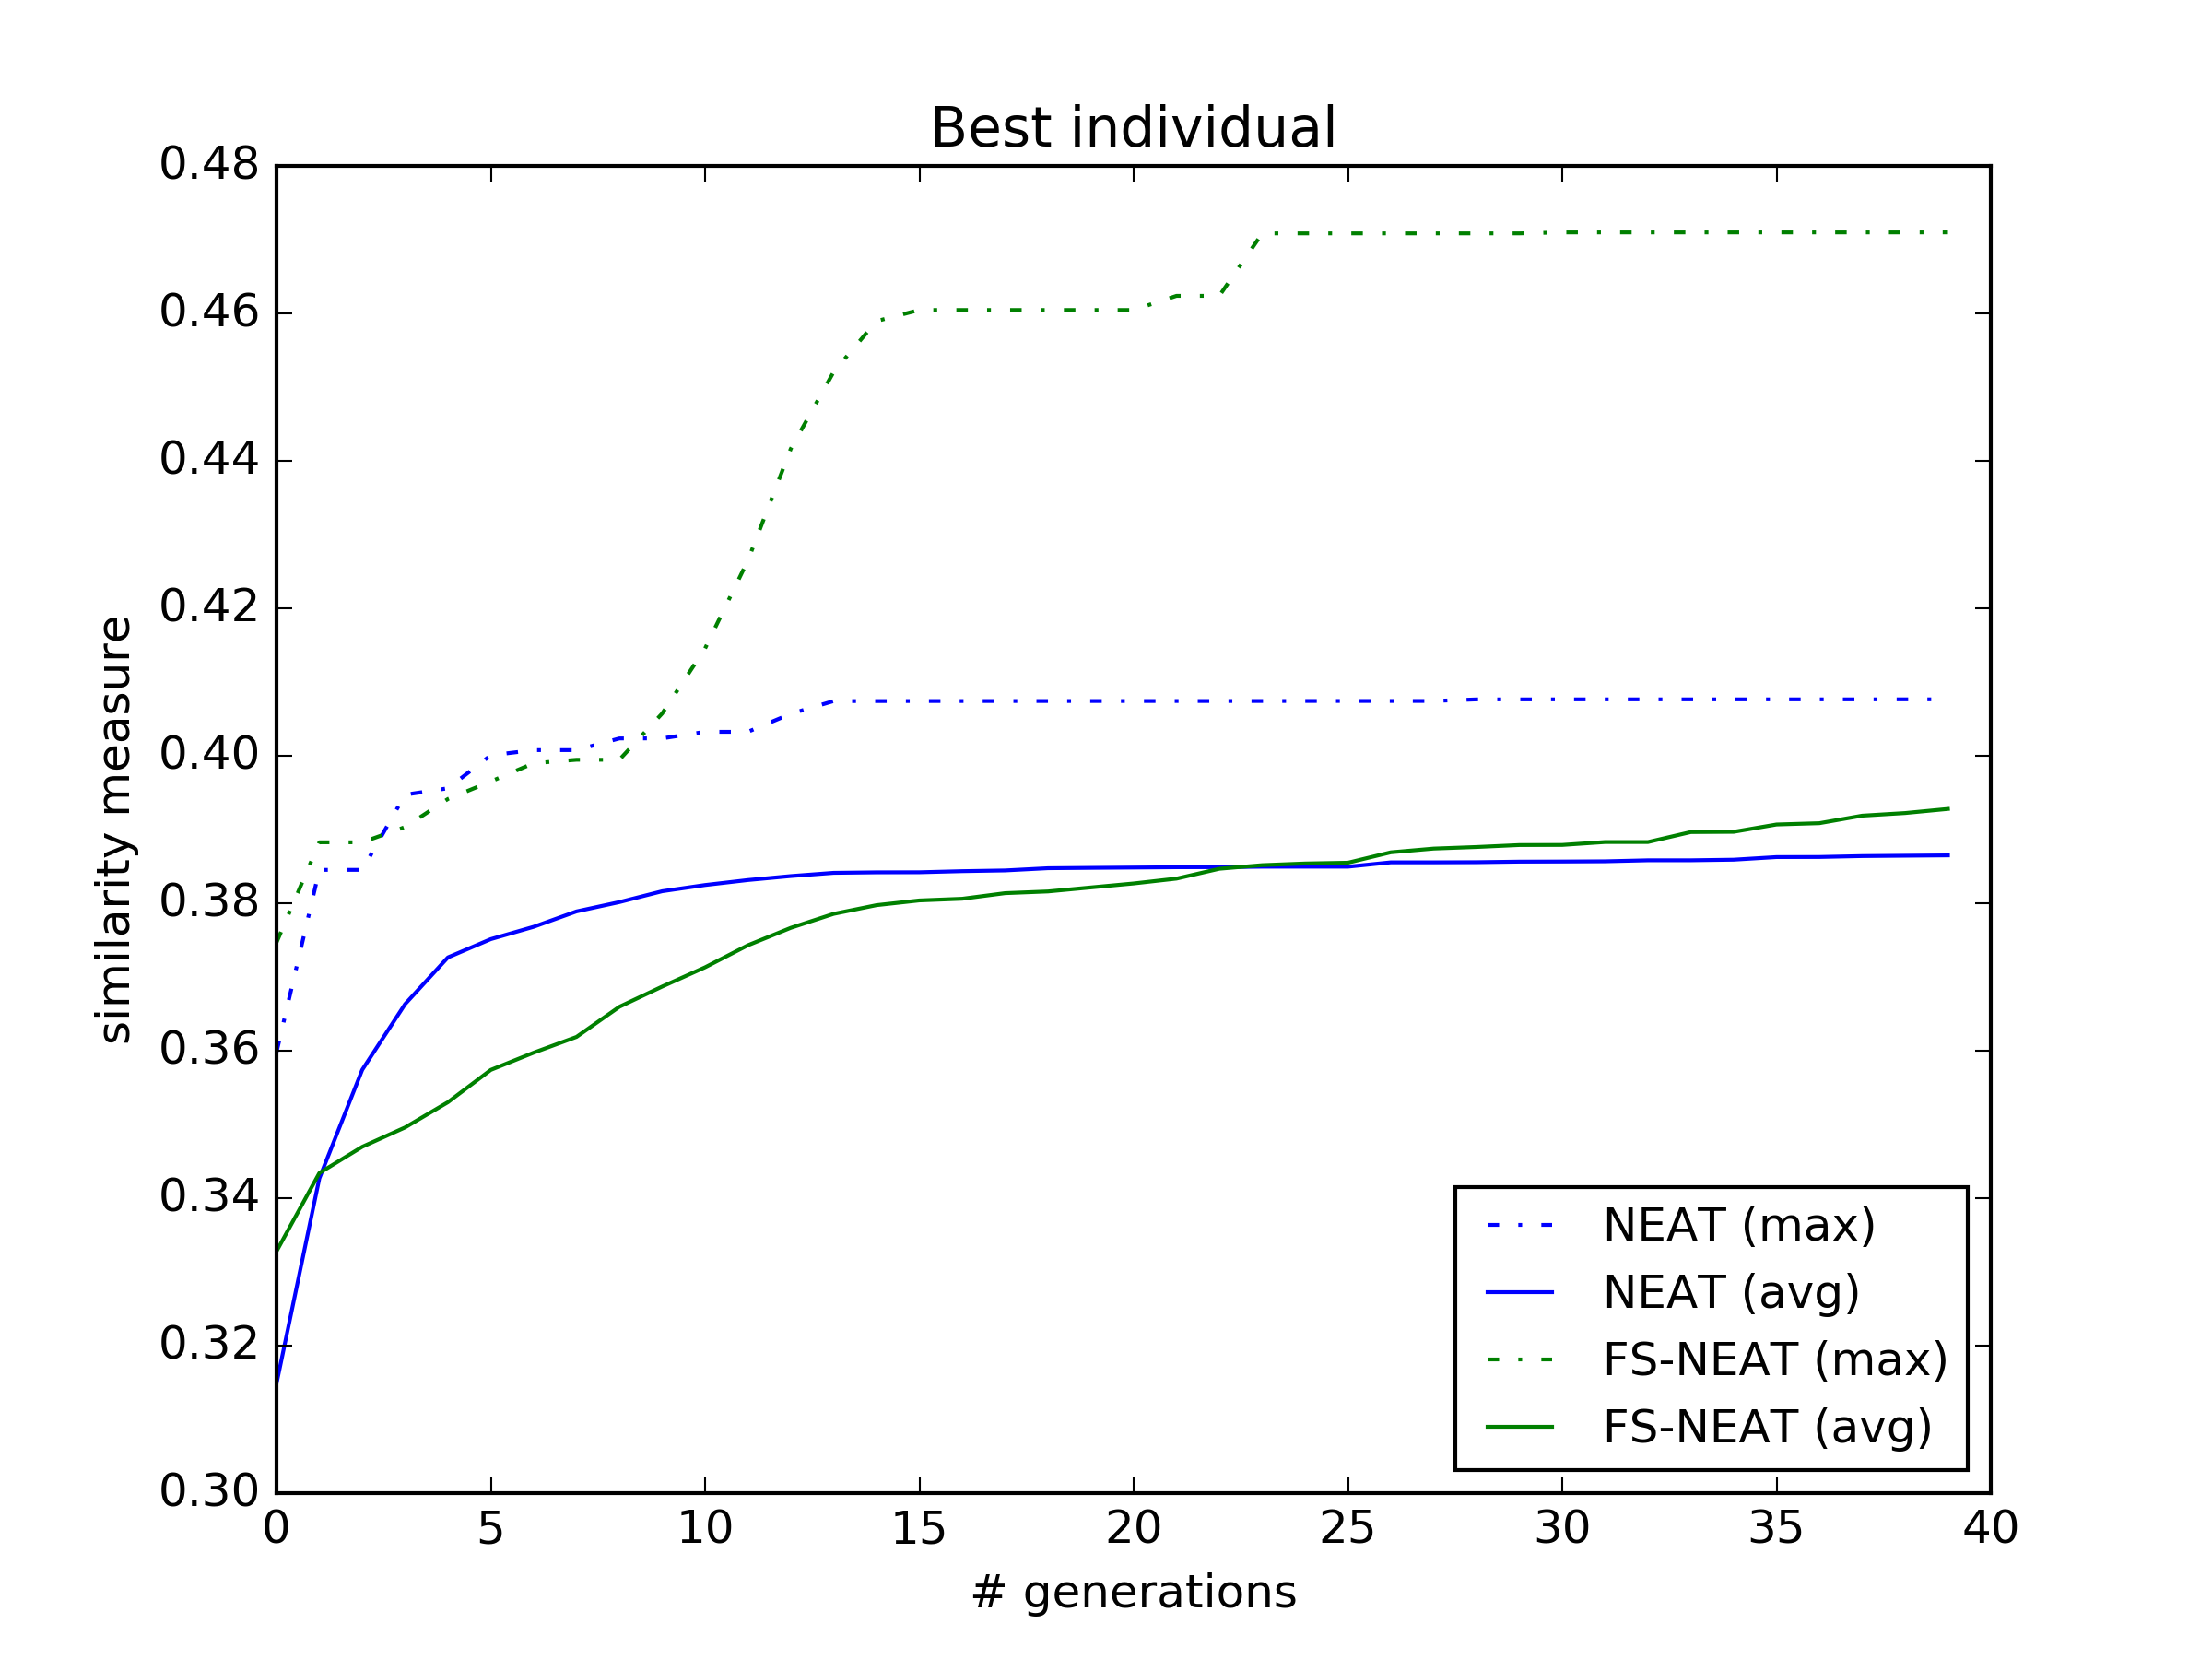
\includegraphics[width=0.85\textwidth]{neat_vs_fs_neat_avg_max}
    \caption{Fitness values in runs with NEAT and FS-NEAT, aggregated from 20 runs with each configuration.}
    \label{fig:neat_vs_fs_neat_avg_max}
\end{figure}



